\section{Interpolation}
When talking about trajectories through conceptual spaces, we refer to interpolation as the use of virtual concepts that factor into the abstraction to the superior space.  Since we formalized conceptual spaces as Hilbert spaces, we can analogously talk about drawing a curve or curve through points in the space.  Hence, the process of interpolation is simply sampling from a regression.

\subsection{Symbol Sparsity}
As discussed in section (?) on segmentation, interpolation is necessary to deal with symbol sparsity in a given segment.  To reiterate, this problem arises due to the use of the Discrete Fourier Transform in the abstraction process.  Since the precision of a signal, either in the time or frequency domains, is determined by the number of non-zero coefficients describing that signal, if the segmentation process results in a relatively short segment, the number of coefficients will be small, and the resulting transformation imprecise.

The way to deal with this imprecision is fill in coefficients in an informed way such that the transform of the signal accurately represents the original signal while maintaining higher precision.  This is valid because we can think of the sparse signal as a sequence of samples from a function, and by intelligently regressing on those samples, we can obtain the representative function.  By interpolating, we are simply drawing more samples from that regressed function to deal with the precision limits of the DFT.

\subsection{Spatial Geometry}
Though interpolation is necessary primarily to deal with symbol sparsity of a segment, it is also the main vehicle in which the geometry of the conceptual space induces the path of the trajectory of symbols.  Since in the Information Dynamics of Thinking, the interpretation of any space is determined by its inner product, we need to interpolate through that space in order to "see" the geometry.

\begin{figure}
  \centering
  \begin{subfigure}[H]{0.45\linewidth}
    \def\svgwidth{\linewidth}
    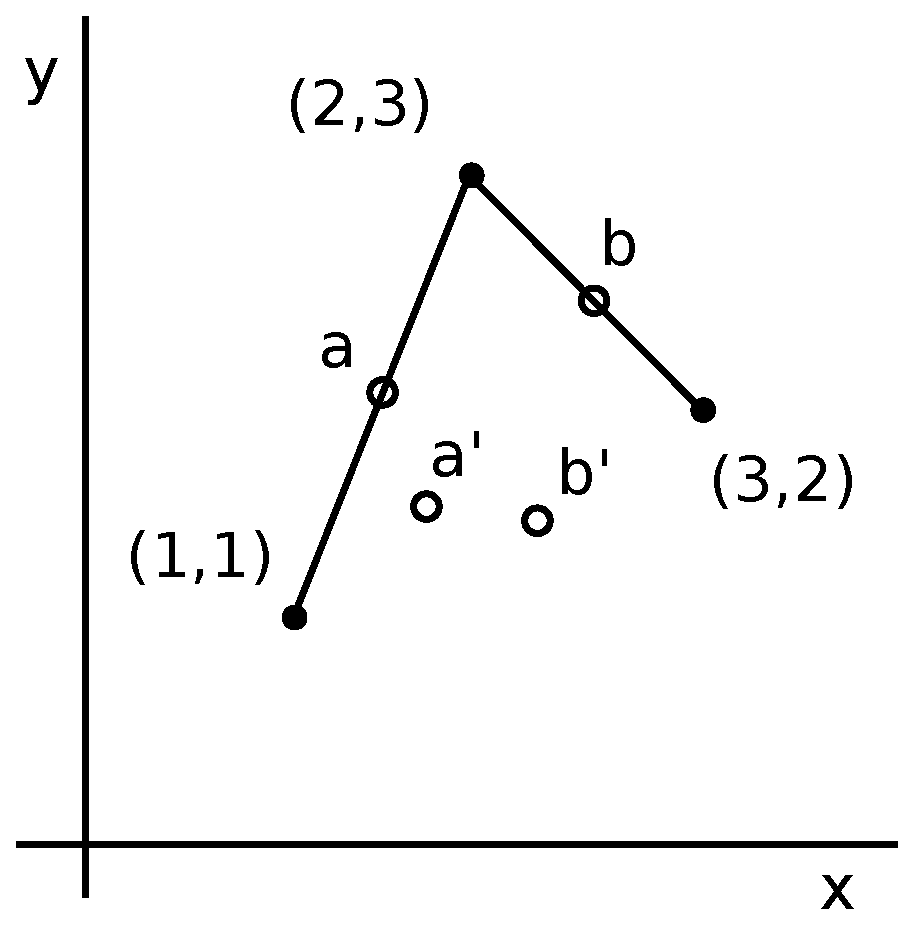
\includegraphics[width=\linewidth]{fig/interpolation-cartesian.eps}
    \caption{Cartesian Trajectory}
  \end{subfigure}
  \begin{subfigure}[H]{0.45\linewidth}
    \def\svgwidth{\linewidth}
    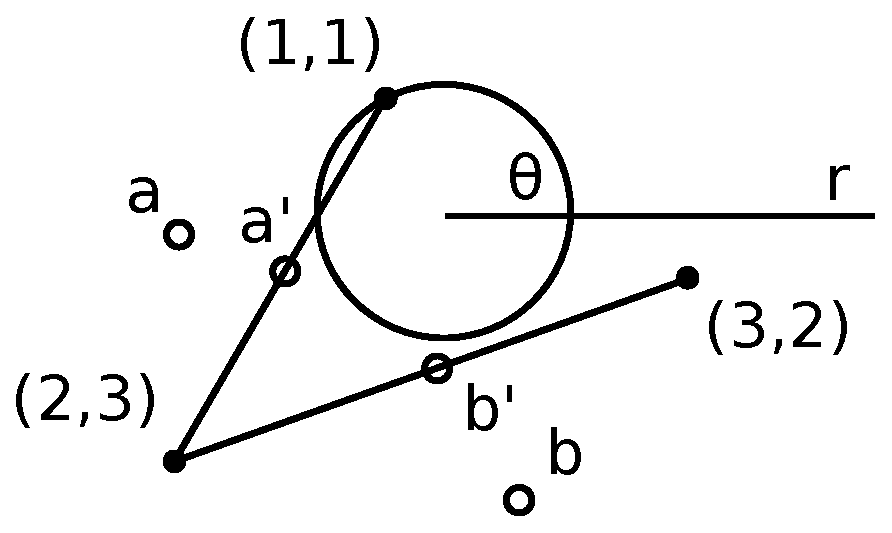
\includegraphics[width=\linewidth]{fig/interpolation-radial.eps}
    \caption{Radial Trajectory}
  \end{subfigure}
  \caption{Example of effect of spatial geometry on interpolation}
\end{figure}

For instance, suppose we have three 2D symbols of which we want to draw a trajectory through. Consider two different spaces for conceiving those points: Cartesian (x, y) and Radial (r, $\theta$). Suppose we take the DFT of three points, i.e. as a trajectory without interpolation, in each of the two spaces.  Since the values of each point are exactly the same for both spaces, when examining the transform, there would be no way to tell which space it came from.  If instead we draw lines through the points and interpolate before taking the transform, we see clearly that the interpolated points differ between the two spaces, and so the transform of each trajectory will also be different.  In this way, the information about the geometry of the space can have an effect on the abstraction of the trajectory in that space.

\subsection{Types}
Since our conceptual spaces are represented as Hilbert spaces, interpolating a trajectory through a sequence of concepts is equivalent to regressing through the points of the space and sampling from that regression.  As such, we can employ any number of regression techniques from the literature to determine an appropriate trajectory.

\subsubsection{Connect the Dots}
Though not really regression per say, the simplest method for interpolating between points would be to just draw a straight line between them and sample from that line.  This method has the benefit of being very simple, and may prove to be near-equivalent to other methods if the number of interpolated points is low enough.

The problem with this method is that it is not continuously differentiable and therefore quite "sharp".  This would manifest in the DFT by resulting in high amplitudes at higher frequencies.  It is difficult to say a priori if this is desirable, but it seems in general that we would prefer smoother functions through these points to avoid this effects.

\subsubsection{Gaussian Regression (Kriging)}
One method for creating a smooth curve through these points is Gaussian Regression.  By thinking of the sequence of points as a multivariate Gaussian distribution, we can think of a distribution of trajectories or functions, i.e. a process, through these points.  By finding the mean function of this process we can find the maximum a posteriori trajectory of the process, resulting in the highest likelihood function through a sequence of points.  This method automatically avoids problems of overfitting inherent in higher-order transformation linear regression methods, though has the problem being computationally expensive.

By utilizing the square exponential kernel for Gaussian regression, the resulting curve will not only by the MAP curve, but also infinitely differentiable, meaning that it is hella smooth.  This smoothness results in a reduction of large high frequency amplitudes that could potentially happen in simpler methods like Connect-the-dots.

